\documentclass[12pt]{article}
\usepackage{hyperref}
\usepackage{authblk}
% Document Layout
\usepackage{natbib}
\bibliographystyle{aer}

\usepackage{geometry} % Customize document dimensions, margins, and page size.
\usepackage{fancyhdr} % Extensive control of page headers and footers.
\usepackage{titlesec} % Control over section and chapter headings.

% Font and Text
\usepackage[utf8]{inputenc} % Allows input of international characters.
\usepackage[T1]{fontenc} % Font encoding.
\usepackage[english]{babel} % Multilingual support.
\usepackage{amsmath, amsfonts, amssymb} % American Mathematical Society packages for advanced math typesetting.
\usepackage{mathptmx} % Times font
\usepackage{helvet} % Helvetica font
\usepackage{courier} % Courier font

% Graphics and Tables
\usepackage{graphicx} % Enhanced support for graphics.
\usepackage{subfigure} % or use \usepackage{subcaption} for handling sub-figures within a single figure environment.
\usepackage{float} % Improved interface for floating objects (tables, figures).
\usepackage{wrapfig} % Allows figures or tables to have text wrapped around them.
\usepackage{pgf, tikz} % Creating high-quality diagrams and figures.
\usepackage{xcolor} % Easy driver-independent access to several kinds of color tints, shades, tones, and mixes of arbitrary colors.
\usepackage{color} 
\usepackage{tabularx} % Enhanced tables.
\usepackage{booktabs} % Publication quality tables in LaTeX.

\usepackage{threeparttable}
\usepackage{longtable}
\usepackage{pdflscape}

% Set the page size and margins
\geometry{letterpaper, portrait, margin=1in}


\title{Sketch for the Conceptual Framework}
\author[1]{Zhiyao (Yao) Ma}
\affil[1]{UC Davis}
\date{\today}


\begin{document}
\maketitle
\tableofcontents
\newpage

% ------------------------------------------ %
% ------------------------------------------ %
% ------------------------------------------ %





% ------------------------------------------ %
% ------------------------------------------ %
% ------------------------------------------ %
\newpage
\section{Traders' Competition: Oligopsonistic Maximization Problem}

To capture the element of time-varying buyer-side competition and incorporate it into the price parameters in the model above, I am considering the Cournot market structure for each trading period from the traders' perspective as follows. 

\subsection{Objective and Profit Function}
In each trading period, each buyer \( i \) aims to maximize their profit \( \pi_i \). The profit for buyer \( i \) is given by:
\begin{equation}
\pi_i = r_i(q_i) - p(Q) q_i
\end{equation}
where:
\begin{itemize}
  \item \( r_i(q_i) \) is the revenue obtained from selling the purchased quantity \( q_i \).
  \item \( p(Q) \) is the inverse supply function representing the price per unit when the total quantity \( Q \) is purchased.
  \item \( q_i \) is the quantity purchased by buyer \( i \).
  \item \( Q \) is the total quantity purchased by all buyers, \( Q = \sum_{j} q_j \).
\end{itemize}

\subsubsection{First-Order Condition (FOC)}
To maximize profit, the buyer will choose \( q_i \) such that the marginal revenue equals the marginal expenditure. The first-order condition (FOC) for maximization is:
\begin{equation}
\frac{\partial \pi_i}{\partial q_i} = \frac{\partial r_i(q_i)}{\partial q_i} - \frac{\partial [p(Q) q_i]}{\partial q_i} = 0
\end{equation}

\subsubsection{Additional Assumptions}
\begin{itemize}
  \item Homogeneous buyers: all buyers are identical.
  \item Perfect Competition in the output market: \( r_i'(q_i) = MR \) (marginal revenue is a constant, MR, for all buyers). Reasoning behind: Although traders may exercise buyer power in localized procurement markets, they then sell into broader output markets and face competition from traders who operate in different regions.
  \item The derivative of \( Q \) with respect to \( q_i \) is given by:
    \begin{equation}
    \frac{\partial Q}{\partial q_i} = 1 + \lambda
    \end{equation}
  \item The quantity purchased by each buyer is:
    \begin{equation}
    q_i = \frac{Q}{n}
    \end{equation}
    where \( n \) is the number of buyers.
  \item The elasticity of supply is:
    \begin{equation}
    \mu = \frac{\partial Q}{\partial p} \cdot \frac{p}{Q}
    \end{equation}
\end{itemize}

\subsubsection{First-Order Condition again}
\begin{equation}
MR = p + \frac{Q}{n} p'(Q) (1 + \lambda)
\end{equation}
Given the elasticity of supply \(\mu\):
\begin{equation}
\mu = \frac{\partial Q}{\partial p} \cdot \frac{p}{Q}
\end{equation}
Inverting to express \(\frac{\partial p}{\partial Q}\):
\begin{equation}
\frac{\partial p}{\partial Q} = \frac{1}{\frac{\partial Q}{\partial p}} = \frac{p}{\mu Q}
\end{equation}
Substitute \( p'(Q) \) into FOC:
\begin{equation}
MR = p + \frac{Q}{n} \cdot \frac{p}{\mu Q} \cdot (1 + \lambda)
\end{equation}
Simplifying:
\begin{equation}
MR = p + \frac{p}{n \mu} \cdot (1 + \lambda)
\end{equation}
\begin{equation}
MR = p \left(1 + \frac{1 + \lambda}{n \mu}\right)
\end{equation}

\subsection{Lerner Index}
\begin{equation}
L = \frac{MR - p}{p} = \frac{1 + \lambda}{n \mu}
\end{equation}

\subsection{Optimal Procurement Price}
Starting from:
\begin{equation}
MR = p \left(1 + \frac{1 + \lambda}{n \mu}\right)
\end{equation}
Solving for \( p \):
\begin{equation}
p = \frac{MR}{1 + \frac{1 + \lambda}{n \mu}}
\end{equation}
Simplify to avoid fraction within a fraction:
\begin{equation}
\textcolor{blue}{p = \frac{MR \cdot n \mu}{n \mu + 1 + \lambda}}
\label{Eq: optimal procure price, general case}
\end{equation}



\subsection{Important Notes}
\begin{enumerate}
    \item \textbf{Cartel Solution:} Cartel solution is NOT an NE for any static game, but it may be NE behavior in any single play of an infinite-horizon repeated game. (by Folk Theorem)
    
    \item \textbf{Why Cournot, instead of Bertrand?} Analogy to \cite{kreps1983quantity}, I can infer that when traders simultaneously and independently receive "downstream orders" for subsequent distribution, and I assume that the capacity level (the quantity of the downstream orders) are public information and traders compete in Bertrand-like price competition, with the supply allocated in Bertrand fashion where the provision that one cannot satisfy more supply than one's order from downstream in the first stage: \\
    "Capacity introduced + Bertrand" $\Longleftrightarrow$ "Cournot".

    \item \textbf{Supply Elasticity:} the village supply to this model should be elastic in both periods, but differ in two periods because farmers have the "outside" selling options differently. 
\end{enumerate}


\subsection{Case 1: Linear Supply Function}

\subsubsection*{Problem Setting}

Each buyer \( i \) aims to maximize their profit \( \pi_i \):
\[
\pi_i = r_i(q_i) - (a + bQ)q_i
\]
where \( p = a + bQ \) is the linear supply function.

\subsubsection*{First-Order Condition}

To maximize profit, the first-order condition (FOC) is:
\[
MR = \frac{\partial r_i(q_i)}{\partial q_i} = a + bQ + b \frac{Q}{n}
\]
Since \( q_i = \frac{Q}{n} \), the total quantity \( Q \) is:
\[
Q = nq_i
\]
Thus, the FOC simplifies to:
\[
MR = a + bQ \left(1 + \frac{1}{n}\right) = a + bQ \left(\frac{n+1}{n}\right)
\]
Rearranging to solve for \( Q \):
\[
MR = a + bQ \left(\frac{n+1}{n}\right)
\]
\[
MR - a = bQ \left(\frac{n+1}{n}\right)
\]
\[
Q = \frac{n(MR - a)}{b(n+1)}
\]

\subsubsection*{Cournot-competition Price}

Substitute \( Q \) back into the supply function:
\[
p = a + bQ
\]
\[
p = a + b \left( \frac{n(MR - a)}{b(n+1)} \right)
\]
\[
p = a + \frac{n(MR - a)}{n+1}
\]
\begin{equation}
    \textcolor{blue}{p = \frac{a + nR}{n+1}}
    \label{Eq: optimal procure price, linear supply case}
\end{equation}
Thus, the farm-gate price that these middlemen offer to farmers becomes an increasing function of the number of traders showing up ($n$), their marginal value product ($MR$), and the farmers' reservation price ($a$).


% ------------------------------------------ %
% ------------------------------------------ %
% ------------------------------------------ %
\newpage
\section{Theoretical Framework}

\subsection{Basic Model Setup}


\begin{table}[H]
\centering
\caption{Economic Environment at Harvest}
\begin{tabular}{lll}
\toprule
\textbf{Item} & \textbf{Symbol (units)} & \textbf{Status at Harvest} \\
\midrule
Harvest quantity & $q$ & known, fixed and normalized to 1 \\
First-period price & $p_1$ & \textbf{observed} \\
Buyer power now & $\theta_1 = \frac{1 - p_1}{p_1}$ & \textbf{unobserved} (inferred from $p_1$) \\
Buyer-power change & $a$ & \textbf{random} \\
Second-period buyer power & $\theta_2 = \theta_1 + a$ & unknown \\
Price function & $p_t = \frac{1}{1 + \theta_t}$, $t=1,2$ & derived \\
Discount factor & $\delta \in (0,1]$ & observed \\
CRRA risk aversion & $\gamma \geq 0$ & observed \\
\bottomrule
\end{tabular}
\end{table}



Consider a representative farmer who produces a fixed quantity \( q \) of Fuji apples. The farmer must decide, at the moment of harvest, what proportion \( s \in [0,1] \) of this harvest to store for sale in the subsequent trading period, while the remainder, \(1 - s\), is sold immediately at the observed price \(p_1\).

The farmer's intertemporal revenue is therefore given by:
\begin{align}
    R_1 &= (1 - s) q p_1, \\
    R_2 &= s q p_2,
\end{align}
where \( p_t \) denotes the price in trading period \( t \).

\subsection{Market Structure and Price Formation}

Prices are determined by the prevailing buyer power \( \theta_t \) in each period, according to the inverse relationship:
\begin{equation}
    p_t = \frac{1}{1 + \theta_t}, \quad t = 1, 2.
\end{equation}

At the time of the harvest, the farmer observes only the first-period price \( p_1 \), from which he implicitly infers current buyer power:
\begin{equation}
    \theta_1 = \frac{1 - p_1}{p_1}.
\end{equation}

However, the second-period buyer power \( \theta_2 \) remains uncertain and evolves according to:
\begin{equation}
    \theta_2 = \theta_1 + a,
\end{equation}
where \( a \) is a stochastic variable capturing intertemporal shifts in buyer power.

Thus, the second-period price \( p_2 \), conditional on the observed price \( p_1 \) and the random shift \( a \), is:
\begin{equation}
    p_2(a) = \frac{p_1}{1 + a p_1}.
\end{equation}

\subsection{Preferences and Objective Function}

Farmers maximize expected discounted utility over two periods. I adopt the Constant Relative Risk Aversion (CRRA) utility function:
\begin{equation}
    U(x) = \begin{cases}
        \frac{x^{1 - \gamma}}{1 - \gamma}, & \gamma \neq 1, \\
        \ln(x), & \gamma = 1,
    \end{cases}
\end{equation}
where \( \gamma \geq 0 \) denotes the degree of relative risk aversion.

Given this preference structure, the farmer’s optimization problem becomes:
\begin{equation}
\label{eq:objective}
    \max_{s \in [0,1]} \left[U\big((1 - s) q p_1\big) + \delta \mathbb{E}_a\big[U\big(s q p_2(a)\big)\big]\right],
\end{equation}
where \(\delta \in (0,1]\) is the subjective discount factor.

\subsection{Analytical Characterization of Optimal Storage}
The farmer’s optimization problem (\ref{eq:objective}) yields the first-order condition (FOC) for an interior solution \( 0 < s < 1 \):
\begin{equation}
    -(1 - s)^{-\gamma}(q p_1)^{1 - \gamma} + \delta s^{-\gamma}\left(q p_1\right)^{1 - \gamma} M(\gamma, p_1) = 0.
\end{equation}
Simplifying and rearranging, I obtain the optimal storage share explicitly as:
\begin{equation}
\label{eq:s_star}
    s^*(\gamma, \delta, p_1) = \frac{\left[\delta M(\gamma, p_1)\right]^{1/\gamma}}{1 + \left[\delta M(\gamma, p_1)\right]^{1/\gamma}}.
\end{equation}
where
\begin{equation}
\label{eq:M_definition}
    M(\gamma, p_1) \equiv \mathbb{E}_a\big[(1 + a p_1)^{\gamma - 1}\big].
\end{equation}

This result clearly delineates how optimal storage depends on risk aversion (\(\gamma\)), discounting (\(\delta\)), observed initial price (\(p_1\)), and the stochastic evolution of buyer power (captured by \(M(\gamma, p_1)\)).

Corner solutions emerge under boundary conditions:
\begin{itemize}
    \item \(s^* = 0\): immediate sale is optimal if \(\delta M(\gamma, p_1) \leq 0\) or is sufficiently low.
    \item \(s^* = 1\): full storage occurs only if \(\delta M(\gamma, p_1)\) is exceptionally high.
\end{itemize}

\subsection{Distributional Assumption for Intertemporal Buyer Power}

Given empirical insights from Fuji-apple smallholders in Central China, I model \(a\) as a truncated normal distribution:
\begin{equation}
    a \sim \text{TruncatedNormal}(\mu, \sigma^2; a_{\text{min}}, a_{\text{max}}),
\end{equation}
with baseline parameters:
\begin{equation}
    \mu = -0.15, \quad \sigma = 0.10, \quad a_{\text{min}} = -0.40, \quad a_{\text{max}} = 0.25.
\end{equation}
These parameters reflect realistic expectations among smallholder farmers regarding seasonal shifts in buyer competition and market access.

\subsection{Simulation}

To explore how smallholder farmers' optimal storage decisions respond to uncertainty in buyer power, I simulate $a \sim \mathrm{TN}(\mu, \sigma^2; [-0.4, 0.25])$, where $\mu \in \{-0.15, -0.05, 0, 0.15\}$ captures different beliefs about the direction of buyer power change (e.g., improved competition vs. increased collusion), and $\sigma \in \{0.05, 0.15\}$ captures the degree of perceived uncertainty. For each combination of $(\mu, \sigma)$, we generate 200{,}000 Monte Carlo draws of $a$.

We simulate optimal storage shares $s^*$ on a grid of discount factors $\delta \in [0.5, 1]$ and risk aversion parameters $\gamma \in [0, 0.5]$. For $\gamma > 0$, the interior solution is characterized by
\[
s^* = \frac{\left[\delta \cdot \mathbb{E}_a[(1 + a p_1)^{\gamma - 1}]\right]^{1/\gamma}}{1 + \left[\delta \cdot \mathbb{E}_a[(1 + a p_1)^{\gamma - 1}]\right]^{1/\gamma}},
\]
where $\mathbb{E}_a[(1 + a p_1)^{\gamma - 1}]$ captures the curvature-adjusted expectation of the second-period price. For the risk-neutral case $\gamma = 0$, the farmer maximizes expected revenue, and the optimal storage decision is a corner solution:
\[
s^*(\gamma = 0) = 
\begin{cases}
1, & \delta \cdot \mathbb{E}_a\left[\frac{1}{1 + a p_1}\right] > 1 \\
0, & \delta \cdot \mathbb{E}_a\left[\frac{1}{1 + a p_1}\right] < 1 \\
\text{any in } [0,1], & \text{if equality holds}
\end{cases}.
\]

The results, visualized in a series of $3$D surface plots (Figure~\ref{Figure: 3D optimal storage share}), show that storage shares increase with the discount factor and decrease with the level of risk aversion in general. When $\mu$ is negative (improved future competition), farmers store more. Greater variance in $a$ amplifies the response to $\gamma$: risk-neutral or mildly risk-averse farmers may still store aggressively due to upside potential, whereas highly risk-averse farmers reduce storage under uncertainty.


\begin{figure}[pht]
\centering
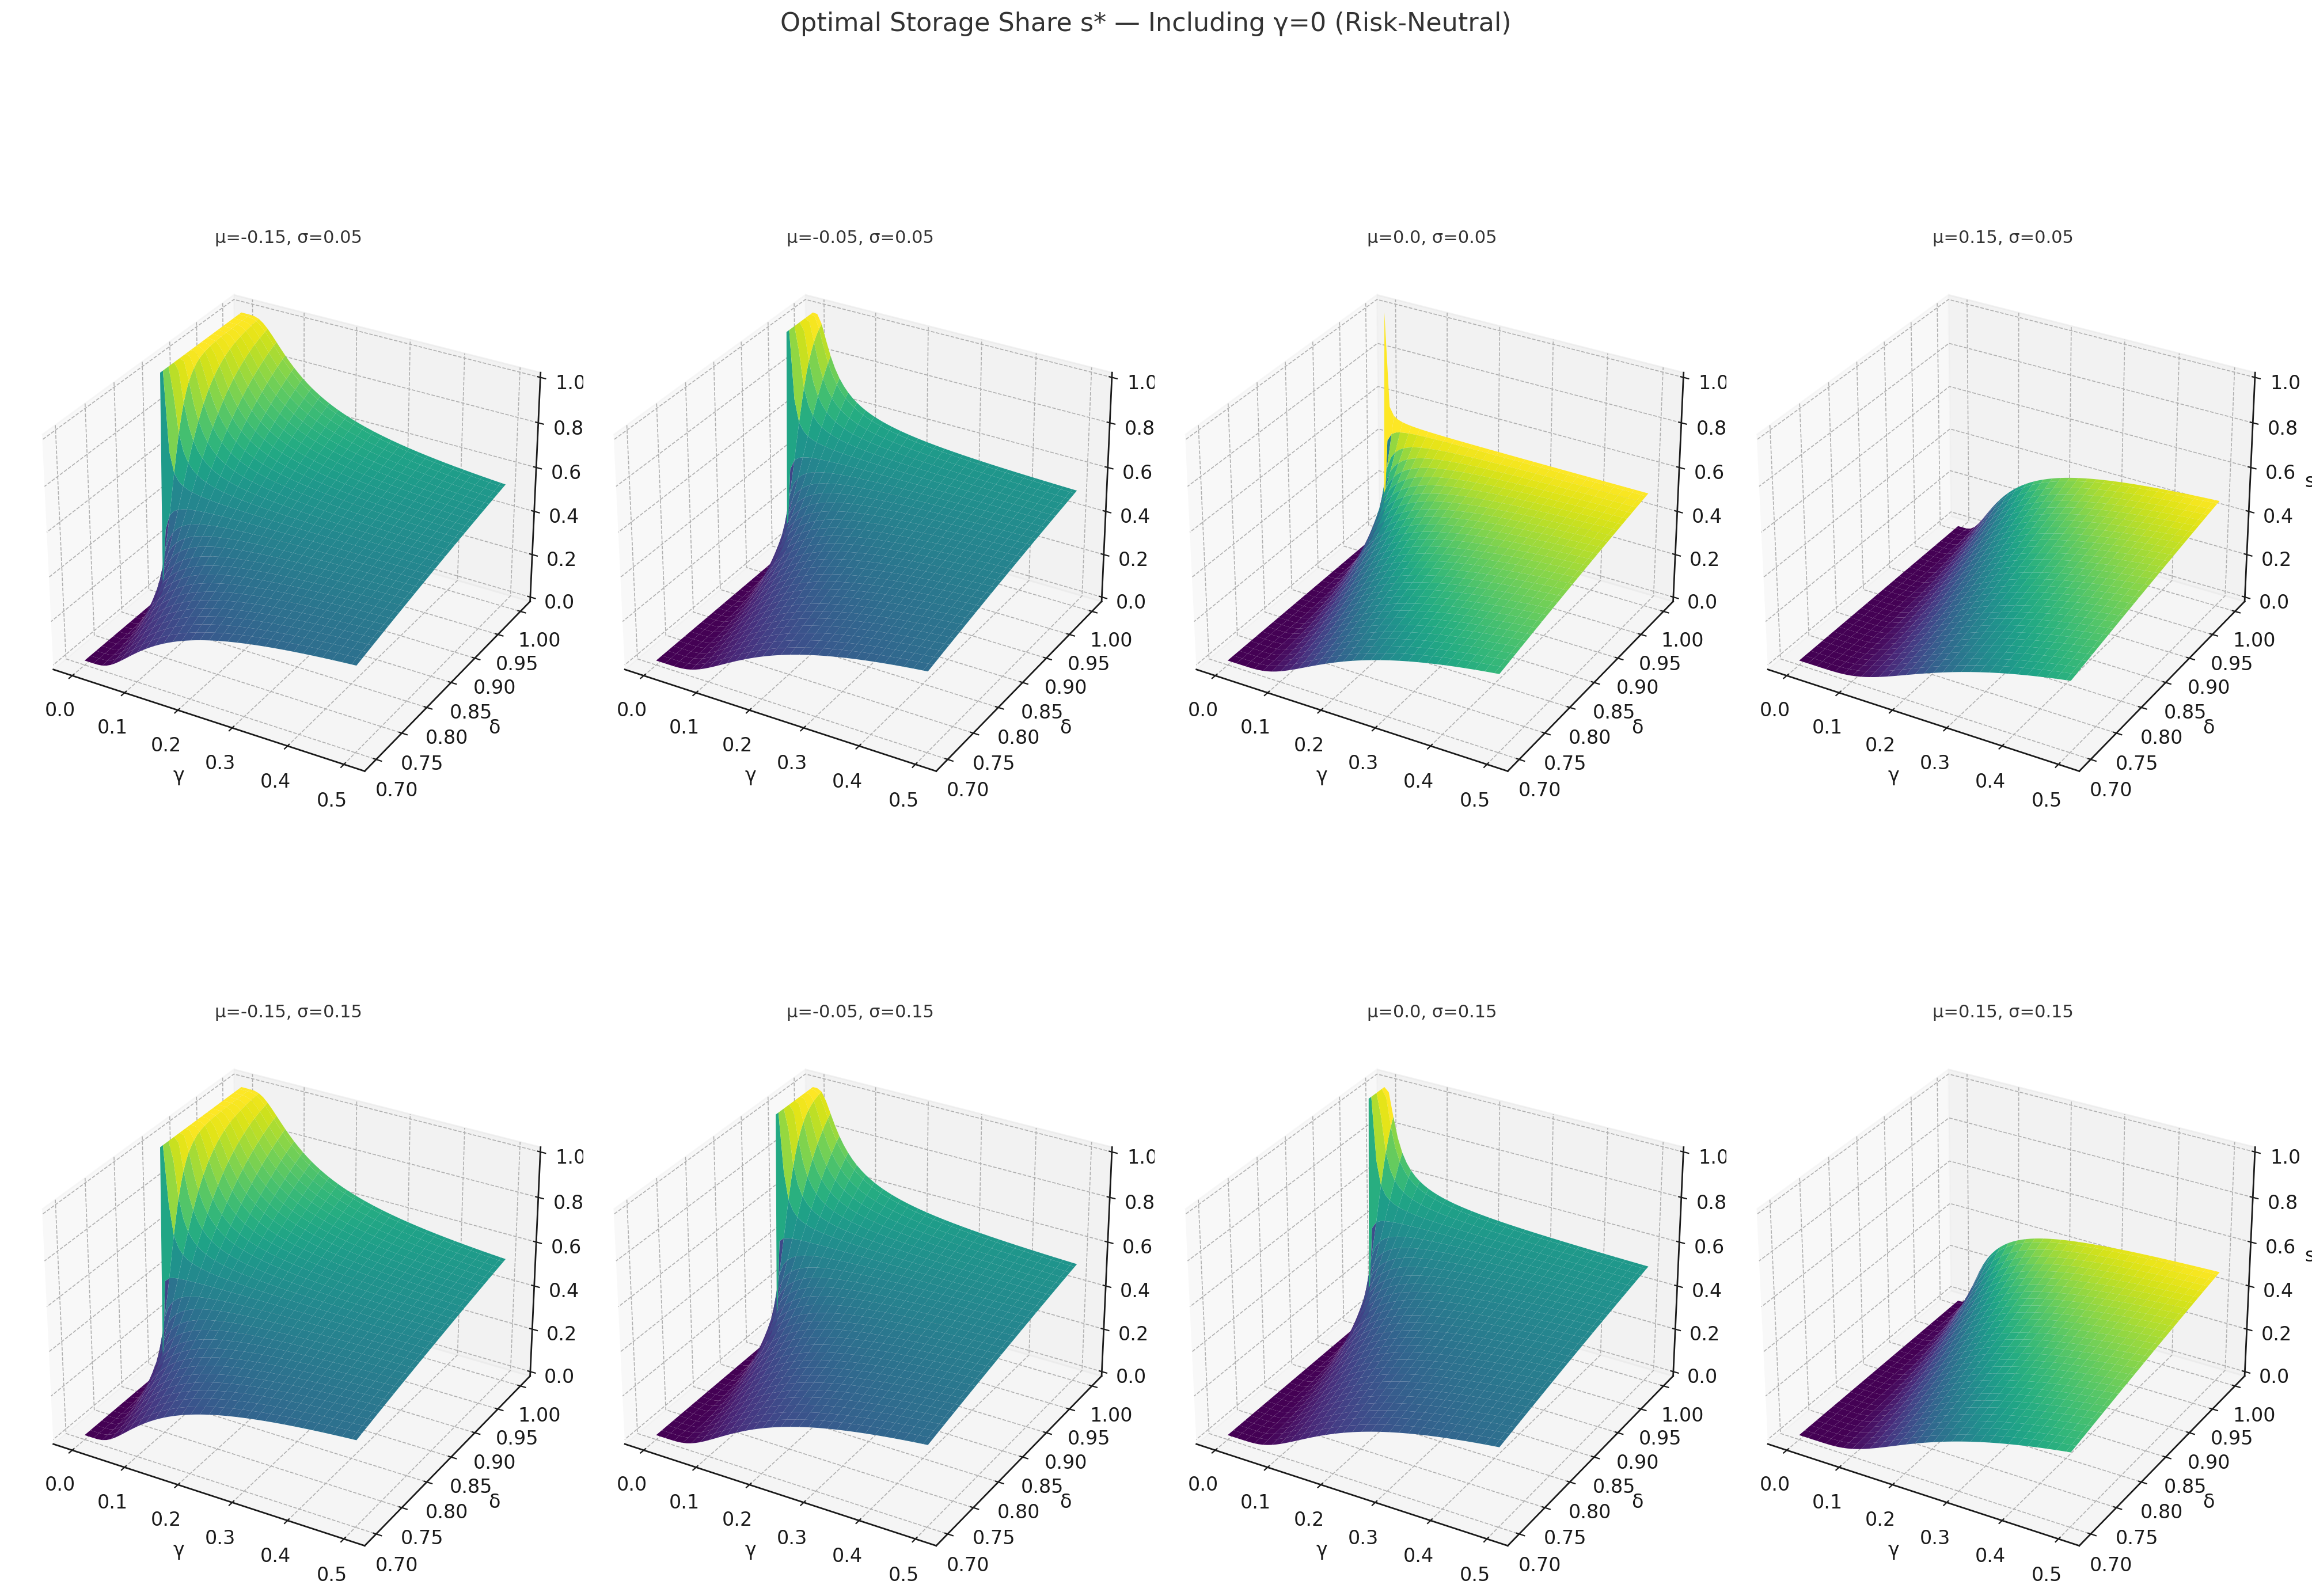
\includegraphics[width=\textwidth]{figures/first_p_0.5_s_optimal.png}
\caption{Optimal Storage Share 3D Visualizations}
\label{Figure: 3D optimal storage share}
\end{figure}



\subsection{Economic Interpretation}

\subsubsection{Effect of Mean Buyer Power Change ($\mu$)}
A negative $\mu$ implies a decline in buyer power over time—interpreted as more competition or trader entry—leading to higher expected second-period prices and increased storage. Conversely, a positive $\mu$ (increasing buyer power) discourages storage.


\subsubsection{Effect of Volatility ($\sigma$)}
Higher variance $\sigma$ increases uncertainty. For risk-neutral farmers, this has no effect. But for risk-averse farmers, greater uncertainty reduces the appeal of storing due to the risk of low future prices.

\subsubsection{Policy Implications}
\begin{itemize}
    \item \textit{Storage Subsidies or Better Storage Technologies}: Low $\delta$ implies farmers are unwilling to delay sales despite good future prices because of the high composite storage cost. Storage subsidies or better Storage technologies would incentivize farmers to adopt storage as an inter-temporal bargaining tool against middlemen.
    \item \textit{Uncertainty management}: Lowering price uncertainty (e.g., through market information platforms or forward contracts) would encourage storage, especially among risk-averse farmers.
\end{itemize}

In summary, the model captures how farmers’ storage behavior responds to intertemporal price expectations, risk preferences, and market volatility. These dynamics have clear implications for rural storage infrastructure, credit access, and trader regulation.











% ------------------------------------------ %
% ------------------------------------------ %
% ------------------------------------------ %
\newpage
\appendix
\section{Previous Try}
\subsection{Numerical Illustration}
\paragraph{Impact of Storage Cost on Storage Decision}
Keeping the prices constant at the same values, Figure explores the impact of varying the discount factor (\( \delta \)) on the optimal storage decision. This graph features three curves, each representing different levels of risk aversion: low ($\gamma=0.1$), moderate ($\gamma=0.3$), and high ($\gamma=0.8$).

As the discount factor ($\delta$) increases, storage becomes less costly (or farmers become more patient), raising the incentive to store for future sales. Consequently, the optimal stored share ($s^*$) consistently increases. 

When the storage cost is reasonably small ($\delta \ge 0.75$), comparing different risk aversion levels, the lowest risk aversion curve ($\gamma=0.1$, yellow) lies above the more risk-averse ones. Less risk-averse farmers store more since they are more comfortable bearing future price uncertainty. Conversely, highly risk-averse farmers ($\gamma=0.8$, red) prefer immediate and certain income.




\subsection{Linking the Model to Empirical Evidence}
The adoption of a constant relative risk aversion (CRRA) utility form here is motivated by two primary considerations. First, empirical evidence consistently shows that individuals' relative risk aversion remains constant across varying levels of wealth \citep{chiappori2011relative}, and the CRRA coefficient, being unitless, facilitates meaningful international comparisons of risk preferences \citep{hardaker2000some}. Second, recent empirical studies conducted in regions closely aligned with my own field sites reinforce this theoretical choice. For example, \cite{jin2024losses} find that apple growers in their surveyed area—which substantially overlaps with my fieldwork locations—exhibit consistent risk-averse behaviors, estimating their CRRA coefficients within the interval of approximately [0.437, 0.575).

My own empirical data, gathered from apple growers in Yanchang County, Central China, indicate an average CRRA coefficient of about 0.3 among the sampled farmers. 

Additionally, within my full sample of 549 apple growers, 200 households (approximately 36.4\%) chose to store all of their produce.


\newpage
\bibliography{reference}




\end{document}